\section{Tracking detectors \label{sec:tracking}}
\subsection[Central drift chamber (Naomi)]{Central drift chamber \label{sec:cdc}}

The Central Drift Chamber (CDC) is a cylindrical straw-tube drift chamber which is used to track charged particles, providing timing and energy loss measurements~\cite{GlueXCDCNIM}.
It is situated inside the Barrel Calorimeter, surrounding the target and start counter, and upstream of the Forward Drift Chambers. 
All of these are inside the solenoid. 
The active volume of the CDC is traversed
by particles coming from the target with polar angles between $6^{\circ}$ and $168^{\circ}$, with optimum 
coverage for polar angles between $29^{\circ}$ and $132^{\circ}$.  

The CDC contains 3522 Mylar\footnote{www.mylar.com} straw tubes of diameter 1.6~cm in $28$ layers,
located in a cylindrical volume which is 1.5~m long, with an inner radius of 10~cm and outer radius of 56~cm, as measured from the beam-line.  
The straws are arranged in 28 layers; 22 of these are axial and 16 are at stereo angles of $\pm 6^{\circ}$ to provide position information in the beam direction. Fig.\,\ref{fig:CDC_stereotubes}  shows the CDC during construction. 

\begin{figure}[tbp]
\begin{center}
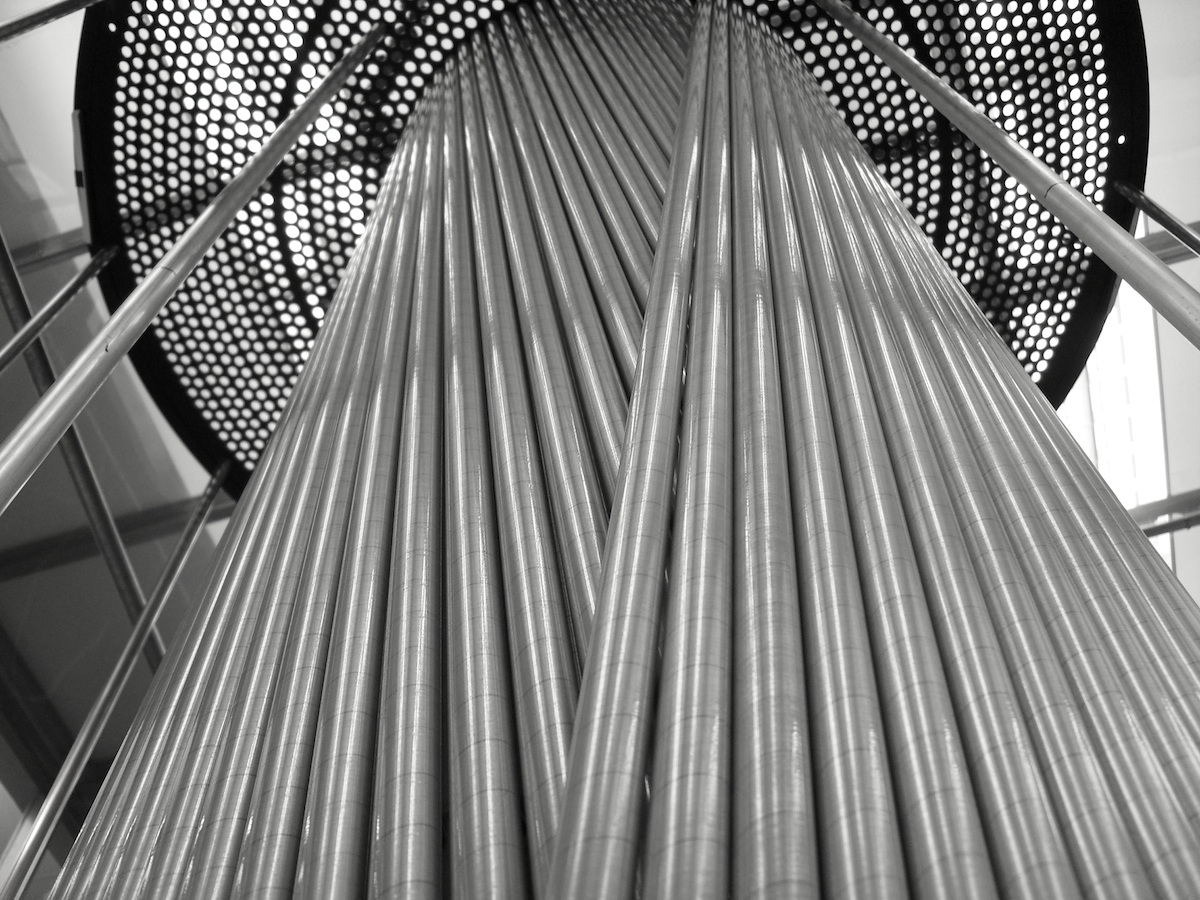
\includegraphics[width=0.7\textwidth]{figures/CDC_stereotubes}  
\caption{\label{fig:CDC_stereotubes}          
  The Central Drift Chamber during construction. A partially completed layer of stereo tubes is shown, surrounding a layer of tubes at the opposing stereo angle. Part of the carbon fiber endplate, some temporary support rods and some of the 12 rods linking the two endplates are also shown.}  
\end{center}
\end{figure}

The volume surrounding the straws is enclosed by an inner cylindrical wall of G10, an outer cylindrical wall of aluminum, and two circular endplates. 
The upstream endplate is made of aluminum, while the downstream endplate is made of carbon fiber. The endplates are connected by 12 aluminum support rods. 
Holes milled through the endplates support the ends of the straw tubes, which are glued into place using several small components per tube.  
These components also support the anode wires, which are 20~$\mu$m diameter gold-plated tungsten, installed with 30~g tension.
At the upstream end these components are made of aluminum and were glued in place using conductive epoxy\footnote{3M Scotch-Weld DP-460NS, www.3m.com}. 
This provides a good electrical connection to the inside walls of the straw tubes, which are coated in aluminum.
The components at the downstream end are made of Noryl plastic\footnote{www.sabic.com} and were glued in place using conventional non-conductive epoxy\footnote{3M Scotch-Weld 920-H, www.3m.com}.
The materials used for the downstream end were chosen to be as lightweight as feasible so as to minimize the energy loss of charged particles passing through them. 

At each end of the chamber there is a cylindrical gas plenum outside the end-plate; the downstream plenum is 2.54~cm deep, with a sidewall of ROHACELL\footnote{www.rohacell.com} and a final outer wall of aluminized Mylar film, and the upstream plenum is 3.18~cm deep, with a polycarbonate sidewall and a polycarbonate disc as its outer wall. 
Five thermocouples are located in each plenum and used to monitor the temperature of the gas.
The gas mixture used is 50$\%$ argon and 50$\%$ carbon dioxide, at atmospheric pressure, with a small admixture of isopropanol to delay aging.
The gas supply runs in 12 tubes through the volume surrounding the straws into the downstream plenum. 
There it enters the straws and flows through them into the upstream plenum. From the upstream plenum the gas flows into the volume surrounding the straws, and from there it exhausts to the outside, bubbling through small jars of mineral oil.

The readout wires pass through the polycarbonate disc and the upstream plenum to reach the anode wires. 
They are connected in groups of 20 to 24 to transition boards which are mounted onto the polycarbonate disc. 
Preamplifiers\cite{hdnote2515} are mounted on high voltage boards which are bolted onto the transition boards. The aluminum endplate, outer cylindrical wall of the chamber, aluminum components connecting the straws to the aluminum endplate and the inside walls of the straws are all connected to a common electrical ground. 
The anode wires are held at +2.1kV during normal operation. 

Fig.\,\ref{fig:CDC_rhs}  shows the CDC during initial readout tests 
\begin{figure}[tbp]
\begin{center}
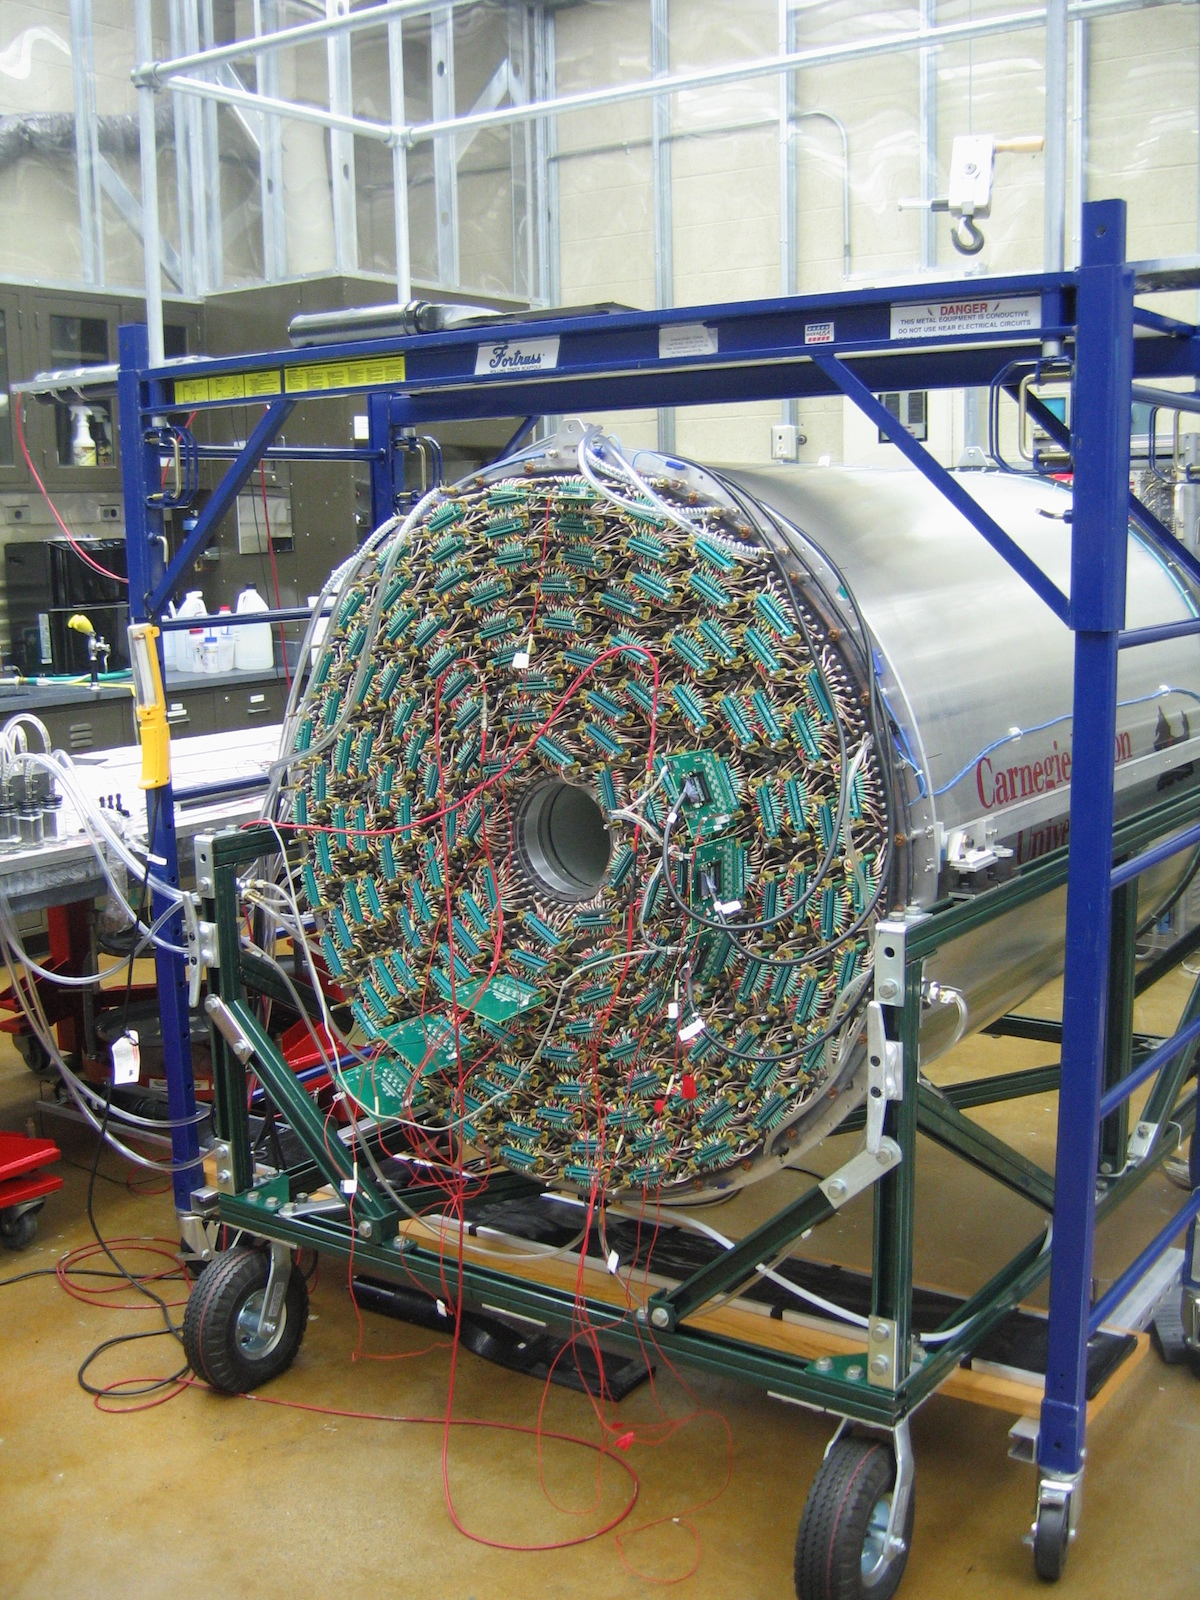
\includegraphics[width=0.7\textwidth]{figures/cdc_rhs.jpg}  
\caption{\label{fig:CDC_rhs}          
  The Central Drift Chamber during initial readout tests. Several HVBs and preamplifiers and many transition boards are visible.}
  \end{center}
\end{figure}


\subsection[Forward drift chambers (Lubomir)]{Forward drift chambers
\label{sec:fdc} }

The Forward Drift Chamber (FDC) system consists of 24 disk-shaped planar drift chambers of 1m-diameter.
They are grouped into four packages inside the bore of the spectrometer magnet.
Due to the high particle density in the forward region the tracking there requires
good multi-track separation.
This is achieved with additional cathode strips on both sides of the wire plane allowing for a  reconstruction of a space point on the track from each chamber. 
The FDC registers tracks with polar angles as low as $1^\circ$ and up to $10^\circ $
with all the chambers, while having partial coverage up to $20^\circ$.

One FDC chamber consists of a wire plane and two cathode planes on both sides at a distance of $5$~mm from the wires (Fig.~\ref{FDC_OneCell}).
\begin{figure}[tbp]
\begin{center}
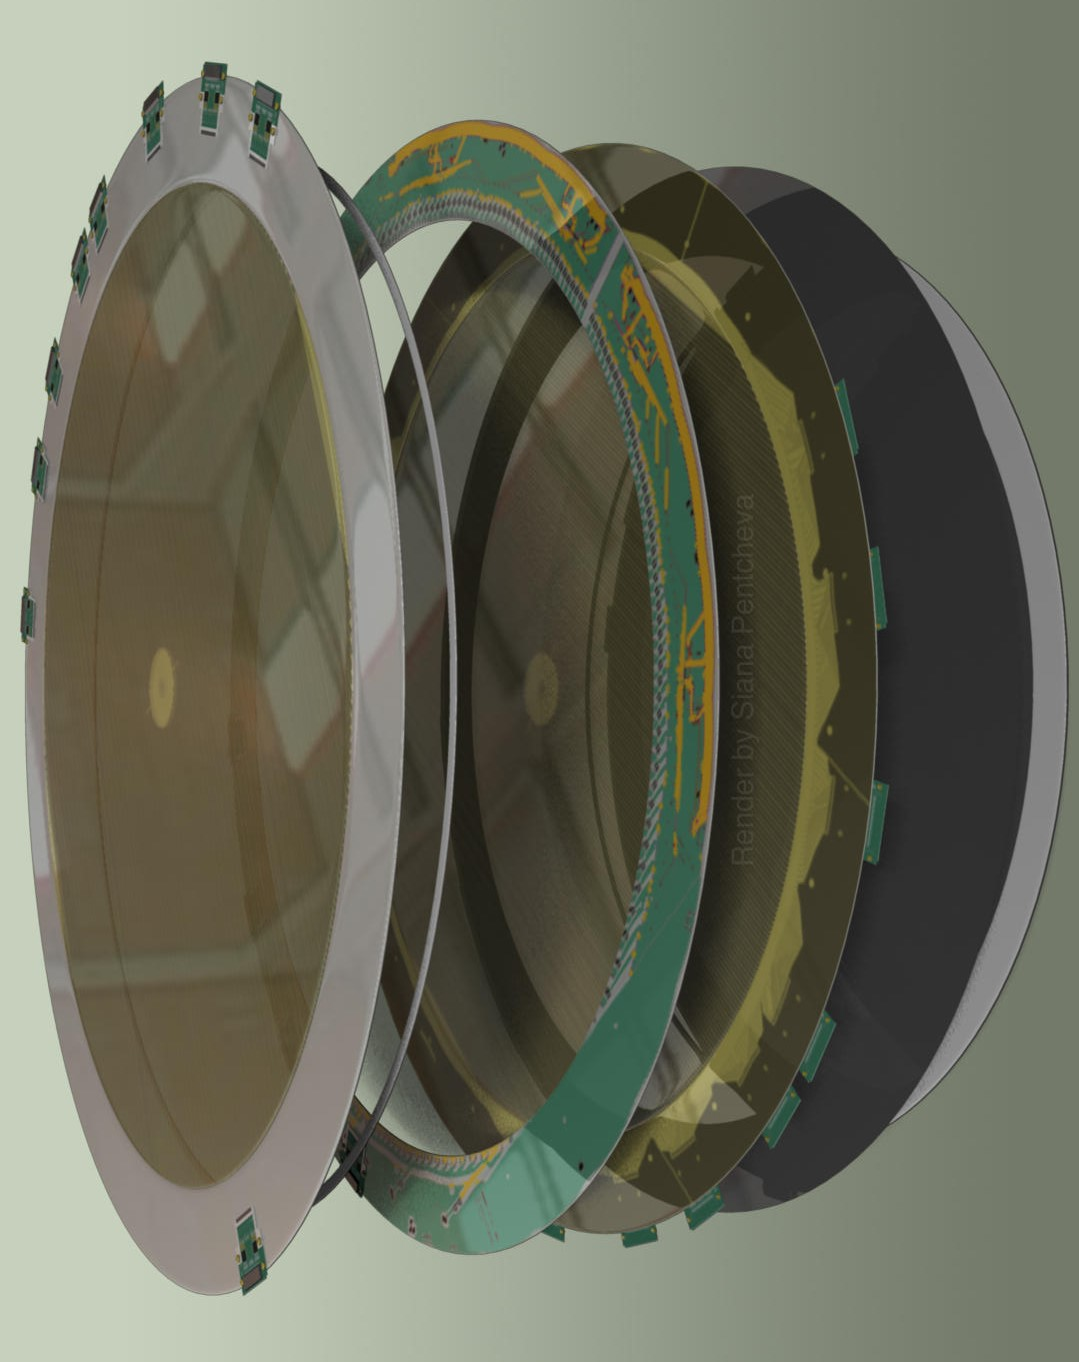
\includegraphics[width=0.75\textwidth]{figures/FDC_OneCell.jpg}  
\caption{\label{FDC_OneCell}
Artistic view of one FDC chamber (from left to right): upstream cathode, wire plane, downstream cathode, chamber separator.
}
\end{center}
\end{figure}
To minimize the material and allow registration of low energy photons by the outside e.m. calorimeters,
the frame that holds the wires is made out of Rohacell with a thin G10 skin.
The wire plane has sense ($20~\mu$m diameter) and field ($80$~$\mu$m) wires $5$~mm apart, forming a field cell of $10\times 10$~mm$^2$. 
The gas mixture used is $40\%$~Ar and $60\%$~CO$_2$.
A positive HV of about $2.2$~kV is applied on the sense wires and negative of $0.5$~kV on the field ones. 
The cathodes are made out of $2$-$\mu$m-thin $Cu$ strips on Kapton foil with a pitch of $5$~mm and are held on ground. The strips on the two cathodes are at $30^\circ $ bewteen each other and at $75^\circ $ and $105^\circ $ angle w.r.t. the wires.

The six chambers of a package are separated by thin aluminized Mylar.
Each chamber is rotated w.r.t. the previous one by $60^\circ $.
The total material of a package in the sensitive area is $0.43\%$~R.L. and about half of that in the area along the beam line that has no copper on the cathodes.
The sense wires in the inner area of $6-7.8$~cm diameter (depending on the distance of the package to the target) are thickened from $20$~$\mu$m to $\sim 80$~$\mu$m which makes them insensitive to the high raters along the beam.
The distance between the first and last package is $169$~cm. 
All the chambers are supplied with gas in parallel. 
In total $2,304$ wires and $10,368$ strips are read using charge pre-amplifiers with $10$~ns peaking time with a gain of $0.77$~mV/fC for the wires and $2.6$~mV/fC for the strips.

\subsection{Electronics \label{sec:dcelectronics}}
The high voltage (HV) supply units used are CAEN A1550P with noise-reducing modules added to each crate chassis. 
The low voltage (LV) supplies are MPOD MPV8008. 
The preamplifiers are a custom JLab design based on an ASIC~\cite{hdnote2515}
with 24 channels per board; they are charge-sensitive, and are capacitatively coupled to the wires in the CDC and FDC and directly coupled to strips in the FDC. 

Pulse information from the CDC anode wires and FDC cathode strips is obtained and read out using 72-channel 125 MHz 12-bit flash ADCs \cite{Visser2008,5873864}. 
Each fADC receives signals from three preamplifiers. 
The signal cables from different regions of the drift chambers are distributed between the fADCs in order to share out the processing load as evenly as possible.  

The fADC firmware is activated by a signal from the GlueX trigger. It then computes the following for the next pulses observed above a given threshold within a given time window: pulse number, arrival time, pulse height, pulse integral, pedestal height immediately before the pulse, and a quality factor indicating if the arrival time is likely to be less accurate than usual. 
Signal filtering and interpolation is used to obtain the arrival time to the nearest 0.8~ns. 
The firmware performs these calculations for the CDC and FDC alike, and uses different readout modes to provide the data with the precision required by the separate detectors. 
For example, the CDC electronics read out only one pulse but requires both pulse height and integral, while the FDC electronics read out up to 4 pulses and do not require pulse integral.  

The FDC anode wires are read out using the GlueX f1TDC\cite{JLAB2002}. 

\subsection[Gas system (Beni)]{Gas system \label{sec:gas}}
Both tracking chambers the CDC and FDC operate with the same type of gases, argon and CO$_{2}$. Since the relative mixture of
the two gases are slightly different for the two tracking chambers the gas system has two separate identical mixing stations. There is one gas supply of argon and CO$_{2}$ for both mixing stations. A limiting opening in the supply
lines provide over-pressure protection to the gas system and filters in the gas lines provide protection against potential
pollution of the gas from the supply. Both gases are mixed together using mass flow controllers (MFC) that can be 
configured
to provide the desired mixing ratio of argon and CO$_{2}$.  The MFC as well as the related control electronics is from
BROOKS Instruments.\footnote{BROOKS Instruments, https://www.brooksinstrument.com/en/products/mass-flow-controllers.}

The mixed gas is filled into storage tanks one for the CDC one for the FDC. Their pressure is
regulated by controlling the operation of the MFCs with a logic circuit based on Allen-Bradley control logics\footnote{Allen-Bradley, https://ab.rockwellautomation.com/}
that are used throughout the experimental hall and keeps
the pressure in the tank between 10 and 12~psi. The tank serves as a reservoir and buffer.
A safety relieve valve on each tank
provides additional protection against over pressure. While the input pressure to the MFC is at 40~psi the pressure after
the MFC is designed to be always below 14~psi above atmospheric pressure. After the mixing tank there is a provision
built into the system to let the gas pass through an alcohol bath to add a small amount to the gas mixture.
This small admixture of alcohol will protect the wire chambers from aging effects caused by radiation exposure from the beam.
This part of the gas system is located above ground in a separate gas shed before the gas mixture is transported
to the experimental hall via polyethylene pipes.

Down in the hall additional MFC allow to specify the exact amount of gas to be provided to the chambers. One for the CDC
and four for the individual FDC packages. The CDC is operated with a flow of 1~l/m while each FDC package is operated with
a flow of 0.1~l/m. To protect the chambers from over-pressure there is a bypass line at the input to the detectors that
is open to atmosphere after a bath of mineral oil. The height of the oil level determines the maximum possible gas pressure at
the input to the chambers. There is a second mineral oil bath at the output to protect against possible air back-flow into
the chamber. Its height of oil above the exhaust line determines the operating pressure inside the chambers.

Pressure tabs are mounted at many places in the gas system to monitor the pressure during operation. Among these are
6 pressure tabs for each FDC chamber to monitor the pressure in each individual plane. The CDC gas pressure is monitored
at the input, the down stream gas plenum and at the exhaust.

There is an additional tab in the exhaust line that can be used to divert some gas from the chamber exhaust to be connected
to an oxygen sensor to test the amount of oxygen in the gas. Too much oxygen in the gas will degrade the gain of
the chambers and reduce the tracking efficiency. The oxygen levels found in the chamber are below 100~ppm. 

\subsection{Calibration, performance and monitoring \label{sec:dccalib}}
Time calibrations for the drift chambers are used to remove the time offset due to the electronics, so that after calibration the earliest possible arrival time of the pulse signals is at 0~ns. These offsets and the function parameters used to describe the relationship between the pulse arrival time and the closest distance between the track and the anode wire are obtained for each session of data-taking. 

The CDC is used to measure dE/dx of tracks over a wide range of polar angles, including recoiling target protons as well as more forward going tracks. Gain calibrations are made to ensure that the dE/dx is consistent between tracking paths through different straws and stable over time. 
The procedure entails matching the position of the minimum ionizing peak for each of the 3522 straws, and then matching the dE/dx at 1.5~GeV/c to the calculated value of 2.0~ keV/cm. This takes place during the early stages of data analysis. Gain calibration for the individual wires is performed each time the HV is switched on and whenever any electronics modules are replaced. Gain calibration for the chamber as a whole is performed for each session of data-taking; these are limited to two hours as the gain is very sensitive to the atmospheric pressure. Position calibrations were necessary to describe the small deflection of the straw tubes midway along their length; these were performed in 2016 and repeated in 2017, with no significant difference found between the two sets of results.  Position resolution from the CDC is of the order of 130~$\mu$m and its detection efficiency per straw is over 98\% for tracks up to 4~mm from the wire. The efficiency decreases as the distance between the track and the wire increases, but the close-packing arrangement of the straw tubes and the large number of straws traversed by each track compensate for this. 

For the FDC system, an internal per chamber calibration process is first performed to optimize the track position information obtained.  
In the FDC the avalanche created around the wire is seen in three projections: on the two cathodes and on the wires.
The drift time information from the wires is used to reconstruct the hit position perpendicular to the wire.
The strip charges from the two cathodes are used to reconstruct the avalanche position along the wire. 
The same strip information can be used to reconstruct the avalanche position perpendicular to the wire which, due to the proximity of the avalanche to the wire, is practically the wire position as illustrated in Fig~\ref{FDC_wires_from_strips}.
\begin{figure}[tbp]
\begin{center}
%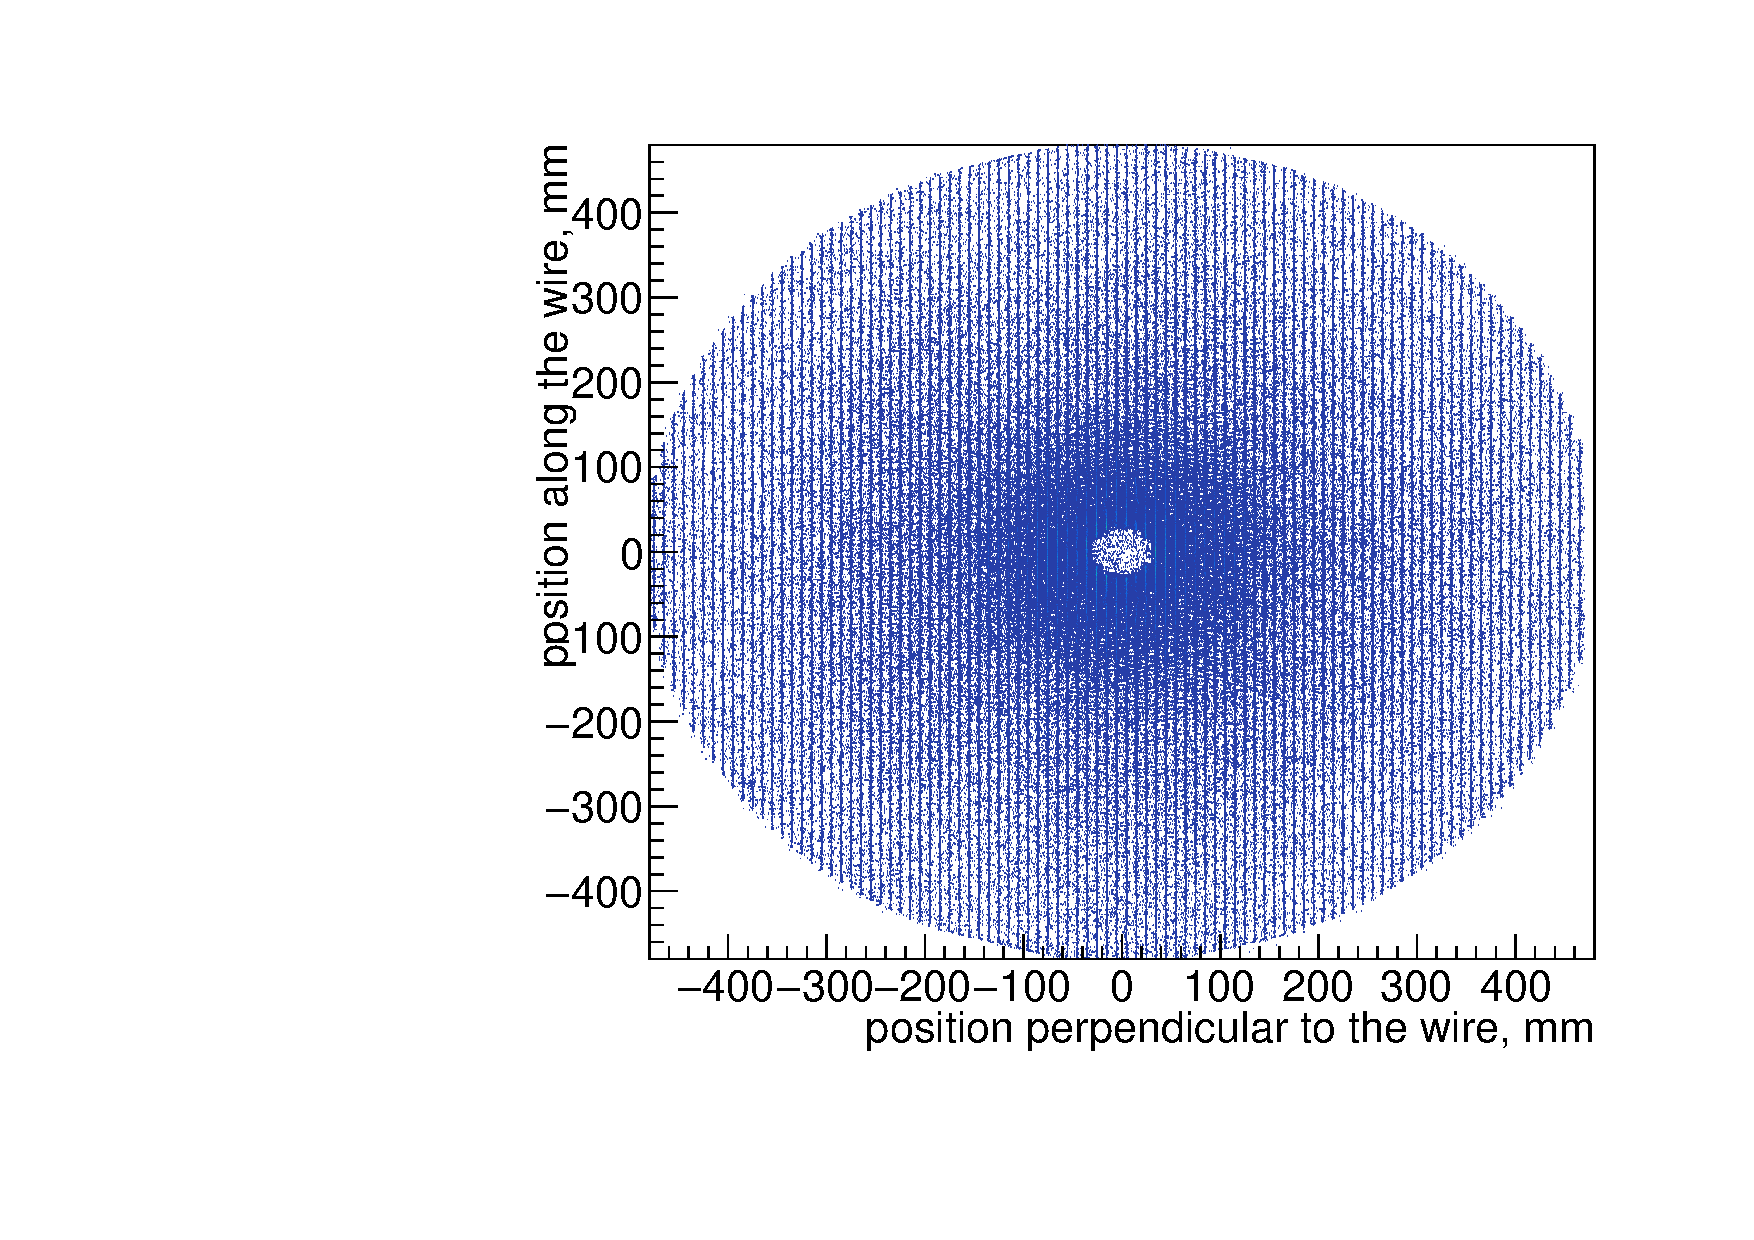
\includegraphics[width=0.95\textwidth]{figures/FDC_wires_from_strips.pdf}  
\caption{\label{FDC_wires_from_strips} Wire (avalanche) positions reconstructed from the strip information on the two cathodes in one FDC chamber.
}   
\end{center}  
\end{figure}
This is used to align the strips on the two cathodes w.r.t. the wires. 
At the same time the residuals of the reconstructed wire positions are an estimate of the strip resolution.
The resolutions of the detector were reported earlier \cite{FDC_NIM}. 
The strip resolution along the wires estimated from the wire position reconstruction, varies between $180$ and $80$~$\mu$m depending on the total charge induced on the strips. The drift distance is reconstructed from the drift time with a resolution between $240$ and $140$~$\mu$m
depending on the distance of the hit to the wire in the $0.5-4.5$~mm range.  

Position offsets and package rotations were determined for both drift chamber systems, first independently, and then together, using the alignment software MILLEPEDE\cite{millepede} in a process described in \cite{GlueXCDCNIM} and in \cite{MikeStaib_thesis}.

Online monitoring software enables the shift-takers to check that the number of channels recording data, the distribution of signal arrival times and the dE/dx are as expected. 




\subsection{Summary \label{sec:dcsummary}}
 
